\newpage
\let\cleardoublepage\clearpage
\part{Информационно-коммуникационные и химические технологии}
\chapter{Информационно-коммуникационные технологии}
\ID{МРНТИ 81.93.29}{https://doi.org/10.58805/kazutb.v.4.25-721}

\begin{articleheader}
\sectionwithauthors{Т.С. Шорманов, А.Т. Мазакова,  М.С. Алиаскар, А.Д. Бургегулов, А.А. Саметова, \linebreak Н.Т. Исимов, Ш.А. Джомартова, Т.Ж. Мазаков}{ПРОГРАММНО-АППАРАТНЫЙ КОМПЛЕКС ДАКТИЛОСКОПИЧЕСКОЙ ИДЕНТИФИКАЦИИ ЧЕЛОВЕКА}

{\bfseries \textsuperscript{1,2}
Т.С. Шорманов, \textsuperscript{2}А.Т.  Мазакова, \textsuperscript{1}
М.С. Алиаскар, \textsuperscript{2}А.Д.
Бургегулов, \textsuperscript{2}А.А. Саметова, \linebreak \textsuperscript{1}Н.Т. Исимов, \textsuperscript{2}Ш.А.
Джомартова, \textsuperscript{1,2}Т.Ж. Мазаков\textsuperscript{\envelope }}
\end{articleheader}

\begin{affiliation}
\textsuperscript{1} Международный инженерно-технологический университет,
Алматы, Казахстан,

\textsuperscript{2} Казахский национальный университет имени аль-Фараби,
Алматы, Казахстан

\raggedright {\bfseries \textsuperscript{\envelope }}Корреспондент-автор: tmazakov@mail.ru
\end{affiliation}

Дактилоскопическая идентификация основывается на уникальности кожных
рисунков на пальцах рук, которые формируются в процессе эмбрионального
развития и не меняются на протяжении жизни человека. Каждый отпечаток
пальца имеет свои особенности, включая линии, завитки, поры, выступы и
другие микроскопические характеристики.

Современные программно-аппаратные комплексы дактилоскопической
идентификации человека обеспечивают высокую точность и скорость
обработки отпечатков пальцев, что делает их востребованными в различных
сферах, таких как правоохранительные органы, система безопасности, а
также в биометрических системах доступа.

В работе рассматривается разработка системы дактилоскопической
идентификации, объединяющей программное обеспечение и аппаратные
компоненты. Предложенная система, основанная на использовании
микроконтроллера Arduino и сканера отпечатков пальцев FPM10A,
предназначена для выполнения операций по хранению, обработке,
идентификации и визуализации данных отпечатков пальцев. Для
идентификации личности были выбраны особенности структуры папиллярных
линий на пальцах рук.

Экспериментальные исследования подтвердили устойчивость разработанной
системы к изменениям масштаба, поворотам изображений и небольшим
искажениям.

{\bfseries Ключевые слова:} биометрические технологии, дактилоскопическая
идентификация, \\программно-аппаратные системы, микроконтроллер.

\begin{articleheader}
{\bfseries АДАМДЫ САУАҚ ІЗІМЕН АНЫҚТАУ ҮШІН БАҒДАРЛАМАЛЫҚ-АППАРАТТЫҚ КЕШЕН}

{\bfseries \textsuperscript{1,2} Т.С. Шорманов, \textsuperscript{2}Ә.Т.
Мазақова, \textsuperscript{1} М.С. Әлиасқар, \textsuperscript{2}А.Д.
Бургегулов, \textsuperscript{2}А.А. Саметова,}

{\bfseries \textsuperscript{1} Н.Т. Исимов, \textsuperscript{2}Ш.А.
Джомартова, \textsuperscript{1,2}Т.Ж. Мазақов\textsuperscript{\envelope }}
\end{articleheader}

\begin{affiliation}
\textsuperscript{1}Халықаралық инженерлік және технология университеті,

\textsuperscript{2}Әл-Фараби атындағы Қазақ ұлттық университеті, Алматы,
Қазақстан,

e-mail:tmazakov@mail.ru
\end{affiliation}

Саусақ ізін анықтау эмбриональды даму кезінде қалыптасатын және адамның
өмір бойы өзгермейтін саусақтардағы тері үлгілерінің бірегейлігіне
негізделген. Әрбір саусақ ізінің өзіндік сипаттамалары бар, соның ішінде
сызықтар, бұйралар, тесіктер, жоталар және басқа микроскопиялық
сипаттамалар.

Адамның саусақ ізін сәйкестендіруге арналған заманауи
бағдарламалық-аппараттық жүйелер саусақ іздерін өңдеудің жоғары дәлдігі
мен жылдамдығын қамтамасыз етеді, бұл оларды құқық қорғау органдары,
қауіпсіздік жүйелері сияқты әртүрлі салаларда, сондай-ақ биометриялық
қол жеткізу жүйелерінде сұранысқа ие етеді.

Жұмыста бағдарламалық және аппараттық құрамдас бөліктерді біріктіретін
саусақ ізін сәйкестендіру жүйесінің дамуы талқыланады. Arduino
микроконтроллерін және FPM10A саусақ ізі сканерін пайдалануға
негізделген ұсынылған жүйе саусақ ізі деректерін сақтау, өңдеу, анықтау
және визуализациялау операцияларын орындауға арналған. Жеке тұлғаны
анықтау үшін саусақтардағы папиллярлық сызықтардың құрылымының
ерекшеліктері таңдалды. Эксперименттік зерттеулер әзірленген жүйенің
масштабтағы өзгерістерге, кескіннің айналуына және шамалы бұрмалануына
тұрақтылығын растады.

{\bfseries Түйін сөздер:} биометриялық технологиялар, саусақ іздерін
сәйкестендіру, \\бағдарламалық-аппараттық жүйелер, микроконтроллер.

\begin{articleheader}
{\bfseries HARDWARE AND SOFTWARE COMPLEX FOR HUMAN DACTYLOSCOPIC
IDENTIFICATION}

{\bfseries \textsuperscript{1,2} T.S. Shormanov, \textsuperscript{2}A.T.
Mazakova, \textsuperscript{1}M.S. Aliaskar, ²A.D.Burgegulov,
\textsuperscript{2}A.A. Sametova,}

{\bfseries \textsuperscript{1}N.T. Isimov, \textsuperscript{2}Sh.A.
Jomartova, \textsuperscript{1,2}T.Zh. Mazakov\textsuperscript{\envelope }}
\end{articleheader}

\begin{affiliation}
\textsuperscript{1} International Engineering and Technology University,
Almaty, Kazakhstan,

\textsuperscript{2} Kazakh National University named after Al-Farabi,
Almaty, Kazakhstan,

e-mail:tmazakov@mail.ru
\end{affiliation}

Fingerprint identification is based on the uniqueness of skin patterns
on the fingers, which are formed during embryonic development and do not
change throughout a person' s life. Each fingerprint has
its own characteristics, including lines, curls, pores, protrusions and
other microscopic characteristics.

Modern software and hardware systems for fingerprint identification of a
person provide high accuracy and speed of fingerprint processing, which
makes them in demand in various areas, such as law enforcement agencies,
security systems, as well as in biometric access systems.

The paper considers the development of a fingerprint identification
system that combines software and hardware components. The proposed
system, based on the Arduino microcontroller and the FPM10A fingerprint
scanner, is designed to perform operations on storing, processing,
identifying and visualizing fingerprint data. The features of the
structure of the papillary lines on the fingers were selected for
personal identification. Experimental studies confirmed the stability of
the developed system to changes in scale, image rotation and minor
distortions.

{\bfseries Keywords:} biometric technologies, fingerprint identification,
hardware and software systems, \\microcontroller.

\begin{multicols}{2}
{\bfseries Введение.} Современные методы защиты информации и объектов
требуют высокой степени надежности, которая зависит от специфики и
уровня безопасности, необходимого в конкретной ситуации. Одним из
наиболее эффективных решений являются биометрические системы, в
частности технологии идентификации личности по отпечаткам пальцев. Эти
системы получили широкое распространение благодаря своей адаптивности,
высокой точности и удобству использования. Применение биометрических
технологий, таких как сканирование отпечатков пальцев, не только
усиливает уровень защиты, но и устраняет необходимость в традиционных
средствах доступа, таких как ключи или карты, заменяя их уникальным,
неизменным биометрическим признаком {[}1{]}.

Дактилоскопические системы функционируют на основе сравнения полученных
отпечатков с хранимыми в базе данных. Методика сопоставления
определяется областью применения технологии. Уникальность отпечатков
пальцев обусловлена анатомическими особенностями строения кожного
рисунка, который формируется под влиянием генетических и экологических
факторов {[}2{]}.

Идентификационные признаки папиллярных узоров делятся на глобальные и
локальные. Глобальные признаки (например, тип узора, направление линий)
видимы невооруженным глазом, в то время как локальные признаки, или
минуции (раздвоения, разрывы и окончания линий), требуют специального
анализа. Методы, основанные на локальных признаках, обладают большей
надежностью и детализированностью, что делает их предпочтительными для
биометрической идентификации. Однако, такие факторы, как давление при
сканировании, влажность кожи и возрастные изменения, могут влиять на
качество изображения отпечатков, что требует использования устойчивых к
искажениям алгоритмов {[}3{]}.

{\bfseries Материалы и методы.} Программно-аппаратные комплексы для
идентификации по отпечаткам пальцев состоят из нескольких ключевых
элементов, которые взаимодействуют друг с другом для реализации
технологии.

\emph{Аппаратные компоненты включают:}

1) Сканеры отпечатков пальцев:

\begin{itemize}[leftmargin=*]
\item
  Оптические сканеры: используют светодиоды (LED) для подсветки пальца и
  камеры для захвата изображения. Это один из наиболее популярных типов,
  однако он может быть подвержен загрязнениям и повреждениям.
\item
  Полимерные (сенсорные) сканеры: используют электрическое поле для
  захвата изображения. Они обеспечивают более высокую точность и
  защищенность от грязи, а также могут быть более компактными.
\item
  Ультразвуковые сканеры: передают ультразвуковые волны на поверхность
  пальца, анализируя отраженные сигналы для создания детализированного
  изображения. Эти сканеры обеспечивают высокую точность, могут работать
  с влажными и поврежденными пальцами.
\item
  Термические сканеры: регистрируют тепловое излучение поверхности
  пальца и могут быть использованы в условиях низкой видимости или при
  загрязненных сканерах.
\end{itemize}

1) Процессоры и устройства обработки: Обработка данных с сенсора требует
быстрого и мощного оборудования для извлечения, анализа и сравнения
отпечатков пальцев в реальном времени. Это может быть либо
специализированное аппаратное обеспечение, либо вычислительные
мощности встроенных процессоров.

Программные компоненты состоят из: 1) Модуля захвата изображений:
Программное обеспечение, отвечающее за захват и обработку изображений
отпечатков пальцев с сенсора. Этот модуль включает в себя алгоритмы для
нормализации изображений, улучшения их качества (например, удаление
шумов, повышение контраста) и подготовки их для дальнейшего анализа.

2) Модуля извлечения признаков: На основе изображения отпечатка пальца
извлекаются ключевые биометрические признаки, такие как:

3) Модуля сопоставления: Алгоритмы сравнивают текущий отпечаток с базой
данных зарегистрированных отпечатков. В случае совпадения система может
подтвердить идентичность, и пользователь получит доступ. Обычно
используются методы, основанные на анализе статистических признаков или
методах машинного обучения для повышения точности и устойчивости к
ошибкам.

4) Модуля идентификации: Этот компонент проверяет, соответствует ли
результат сопоставления зарегистрированным данным пользователя и
принимает решение о подтверждении или отклонении идентификации
{[}4-5{]}.

{\bfseries Обсуждение и результаты.} Традиционные методы контроля доступа,
такие как использование паролей или ключей, часто неудобны и подвержены
риску утраты {[}6{]}.

В ходе данной работы разработана биометрическая система идентификации,
основанная на использовании сканера отпечатков пальцев и
микроконтроллера Arduino. Применение библиотеки Adafruit для Arduino
позволило интегрировать аппаратные и программные компоненты, обеспечив
точное распознавание и идентификацию.

На рисунке 1 представлена фотография разработанного
программно-аппаратного комплекса системы: 1) сканер FPM10A, 2)
микроконтроллер Arduino, 3) средство визуализации результата
распознавания, 4) внешний аккумулятор (Power Bank), 5)
мульти-разветвитель USB.

Программно-аппаратный комплекс состоит из нескольких ключевых
компонентов:

\emph{1) аппаратная часть:}

\begin{itemize}[leftmargin=*]
\item
  оптический сканер FPM10A, способный сохранять до 1000 отпечатков
  пальцев:
\item
  микроконтроллер Arduino, обеспечивающий обработку данных в реальном
  времени.
\end{itemize}

\emph{2) программная часть:}

\begin{itemize}[leftmargin=*]
\item
  библиотека Adafruit\_Fingerprint, позволяющая выполнять все этапы
  обработки отпечатков;
\item
  модули для извлечения ключевых точек и анализа биометрических данных.
\end{itemize}

\emph{3) система электрообеспечения:}

\begin{itemize}[leftmargin=*]
\item
  внешний аккумулятор Power Bank емкостью 10 000 мА, обеспечивающий
  бесперебойную работу комплекса;
\item
  мульти-разветвитель USB, позволяющий снизить энергетическую нагрузку
  на микроконтроллер;
\item
  солнечная панель с контроллером заряда, обеспечивающие зарядку
  внешнего аккумулятора.
\end{itemize}
\end{multicols}

\begin{figure}[H]
    \centering
    \begin{subfigure}[t]{0.4\textwidth} % Align at the top
        \centering
        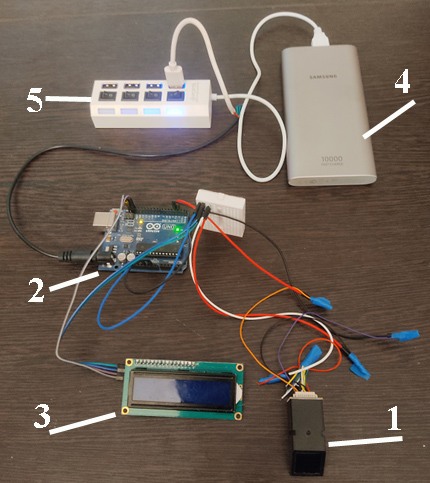
\includegraphics[width=\textwidth]{media/ict/image1}
        \caption*{Рис.1 - Программно-аппаратный комплекс идентификации личности по отпечаткам пальцев}
    \end{subfigure}
    \hspace{0.05\textwidth} % Adjust horizontal space between the subfigures
    \begin{subfigure}[t]{0.4\textwidth} % Align at the top
        \centering
        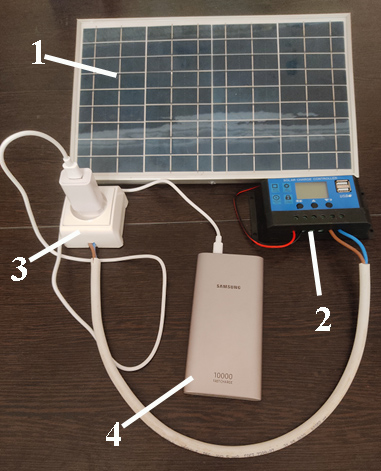
\includegraphics[width=\textwidth]{media/ict/image2}
        \caption*{Рис.2 - Схема электрического обеспечения: 1- солнечная панель, 2) контроллер заряда, 3) розетка для заряда внешнего аккумулятора, 4) внешний аккумулятор}
    \end{subfigure}
\end{figure}

\begin{multicols}{2}
Сенсор использует алгоритмы, позволяющие хранить, обрабатывать и
сопоставлять отпечатки пальцев. Для этого применяется библиотека
Adafruit\_Fingerprint, которая включает функции:

\begin{itemize}[leftmargin=*]
\item
  Захвата изображения.
\item
  Извлечения ключевых признаков (локальных точек).
\item
  Сравнения текущего отпечатка с сохранёнными образцами.
\end{itemize}

Программные инструменты позволяют записывать новые отпечатки, присваивая
каждому уникальный ID (который сохраняется в памяти сенсора для
дальнейшего сравнения), и проверять работу системы через окно серийного
монитора Arduino.

Запись новых отпечатков через программу для Windows

Для записи новых данных в память оптического датчика отпечатков пальцев
рекомендуется использовать специализированную программу для Windows.

На рисунке 3 продемонстрирована работа программно-аппаратного комплекса
по идентификации личности по отпечаткам пальцев.

Внешний аккумулятор Samsung EB-P1100C емкостью 10000 мАч позволяет
работать программно-аппаратному комплексу больше 48 часов (двое суток),
что подтверждается дальнейшими расчетами.

Расчет времени работы Arduino Uno от внешнего аккумулятора Power Bank на
10000 мАч, необходимо учитывать несколько факторов:

Arduino Uno обычно потребляет от 30 до 50 мА при обычной работе (без
дополнительных устройств). При использовании дополнительных модулей,
датчиков или экранов потребление может увеличиться, но для базового
расчета возьмем среднее значение 50 мА.
\end{multicols}

\begin{figure}[H]
	\centering
	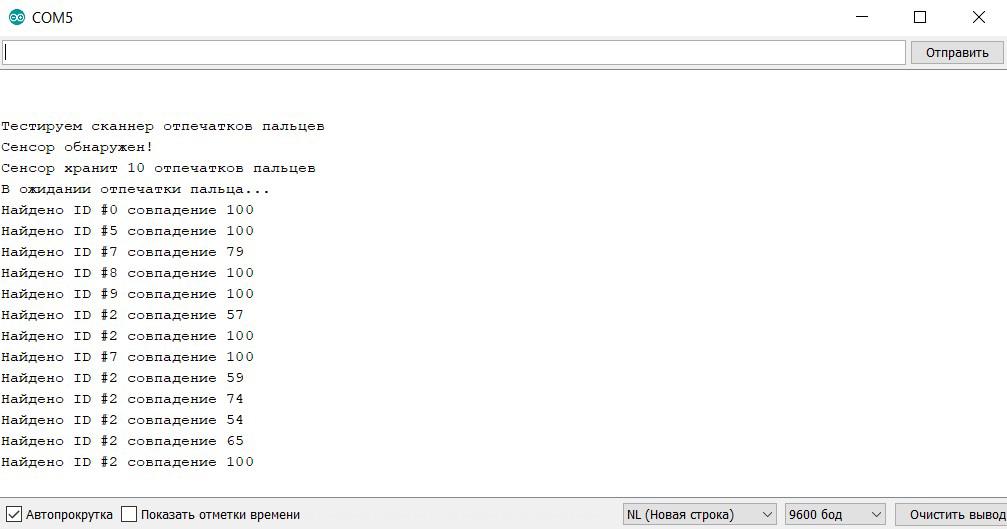
\includegraphics[width=0.9\textwidth]{media/ict/image3}
	\caption*{Рис.3 - Результаты работы программно-аппаратного комплекса}
\end{figure}

\begin{multicols}{2}
Power Bank на 10000 мАч, как правило, имеет выходное напряжение 5 В (при
использовании USB-выхода), и его реальная емкость может быть немного
меньше из-за потерь при преобразовании напряжения. Обычно можно
рассчитывать на эффективность около 85\%. Поэтому примем что эффективная
емкость Power Bank будет примерно 8500мАч

Время работы рассчитывается по формуле:

Время=Емкость / Потребление=8500 мАч / 50 мА=170 часов.

Учитывая, что Arduino подключает дополнительные устройства (датчики,
экраны и т.д.) потребление энергии может увеличиться втрое. Поэтому мы
берем за гарантийное время - 48 часов.

{\bfseries Выводы.} В рамках данной работы получены следующие результаты:

Проведен анализ методов биометрической идентификации, включающих
использование сканеров отпечатков пальцев и алгоритмов сопоставления.

Разработан программно-аппаратный комплекс на основе микроконтроллера и
оптического сканера, обеспечивающий хранение, обработку и идентификацию
отпечатков пальцев. Основой идентификации послужила структура
папиллярных узоров.

Экспериментальные исследования продемонстрировали, что разработанная
система обеспечивает:

1) Устойчивость к изменениям масштаба и поворотам изображения.

2) Инвариантность к незначительным искажениям и изменению уровня
освещения до 50--70\%.

3) Надежное распознавание даже при использовании частичных отпечатков
пальцев.

Преимущества применения дактилоскопической информации:

1) Высокая точность: Отпечатки пальцев имеют уникальные биометрические
признаки, которые остаются неизменными на протяжении всей жизни
человека, что делает их надежным средством для идентификации.

2) Удобство использования: Сканирование отпечатков пальцев требует всего
лишь прикосновения к сенсору, что делает процесс аутентификации быстрым
и удобным.

3) Высокий уровень безопасности: Трудно подделать отпечатки пальцев, что
делает этот метод биометрической идентификации более безопасным по
сравнению с паролями или PIN-кодами.

Особую перспективу представляет разработка алгоритмов для поиска по
неполным отпечаткам пальцев, что особенно важно в реальных условиях,
когда доступна лишь часть изображения для идентификации.

\emph{{\bfseries Финансирование}. Работа выполнена за счет средств НИИ
математики и механики при КазНУ имени аль-Фараби и грантового
финансирования научных исследований на 2023--2025 годы по проекту
AP19678157}.
\end{multicols}

\begin{center}
{\bfseries Литература}
\end{center}

\begin{references}
1. Болл Р.М., Коннел Дж.Х., Панканти Ш. и др. Руководство по биометрии.
-- Москва: Техносфера, 2007.-368 с.
\href{https://www.libex.ru/qna/ref/isbn/}{ISBN}: 978-5-94836-109-3.
URL: https://www.technosphera.ru/lib/book/187

2. Мазур Е.С. Дерматоглифика в исследованиях личности криминалистический
и судебно-медицин\-ский аспекты. -- Томск: Изд. дом ТГУ, 2014, - 150с.
\href{https://www.libex.ru/qna/ref/isbn/}{ISBN}: 978-5-94621-450-6. --

URL: https://ibooks.ru/bookshelf/380802/reading

3. Лепихова Д.Н., Гудков В.Ю., Кирсанова А.А. Обзор современных моделей
представления дактилоскопических изображений // Вестник ЮУрГУ. Серия:
Вычислительная математика и информатика.- 2018.-Т.7(1)- с.40-59.
DOI 10.14529/cmse180104.

4. Гридчин А.В. Микродатчики и микросистемы. -- Москва, Вологда:
Инфра-Инженерия, 2023. -184 с. \href{https://www.libex.ru/qna/ref/isbn/}{ISBN} 978-5-9729-1220-9.
URL: https://www.iprbookshop.ru/133049.html

5. Апейников А.Ф., Гридчин В.А., Цапенко М.П. Датчики (перспективные
направления развития). -- Новосибирск: Изд-во НГТУ, 2001.-176.
\href{https://www.libex.ru/qna/ref/isbn/}{ISBN} 5-7782-0300-4

6. Бриллиант К. Цифровая модель человека. -- М.: Кудиц-образ, 2004.- 400
с. ISBN 5-7782-0300-4
\end{references}

\begin{center}
{\bfseries References}
\end{center}

\begin{references}
1. Boll R.M., Konnel Dzh.H., Pankanti Sh. i dr. Rukovodstvo po
biometrii. -- Moskva: Tehnosfera, 2007.-368 s. ISBN: 978-5-94836-109-3.
URL: {https://www.technosphera.ru/lib/book/187}. {[}in Russian{]}

2. Mazur E.S. Dermatoglifika v issledovanijah lichnosti
kriminalisticheskij i sudebno-medicinskij aspekty. - Tomsk: Izd. dom
TGU, 2014, - 150s. ISBN: 978-5-94621-450-6.

URL: {https://ibooks.ru/bookshelf/380802/reading}/ {[}in Russian{]}

3. Lepihova D.N., Gudkov V.Ju., Kirsanova A.A. Obzor sovremennyh modelej
predstavlenija daktiloskopi\-cheskih izobrazhenij // Vestnik JuUrGU.
Serija: Vychislitel' naja matematika i informatika.-
2018.-T.7(1)- s.40-59. DOI 10.14529/cmse180104. {[}in Russian{]}

4. Gridchin A.V. Mikrodatchiki i mikrosistemy. -- Moskva, Vologda:
Infra-Inzhenerija, 2023. -184 s. ISBN 978-5-9729-1220-9. URL:
https://www.iprbookshop.ru/133049.html.

5. Apejnikov A.F., Gridchin V.A., Capenko M.P. Datchiki (perspektivnye
napravlenija razvitija). -Novosib\-irsk: Izd-vo NGTU, 2001.-176. ISBN
5-7782-0300-4. {[}in Russian{]}

6. Brilliant K. Cifrovaja model'{} cheloveka. -- M.:
Kudic-obraz, 2004.- 400 s. ISBN 5-7782-0300-4. {[}in Russian{]}
\end{references}

\begin{authorinfo}
\hspace{1em}\emph{{\bfseries Сведение об авторах}}

Т.С. Шорманов-- докторант КазНУ имени аль-Фараби, старший преподаватель
МИТУ, Алматы, Казахстан, \linebreak e-mail\href{mailto:shormanov@gmail.com}{\nolinkurl{shormanov@gmail.com}};

А.Т. Мазақова -- докторант КазНУ им.аль-Фараби, e-mail:
\href{mailto:aigerym97@mail.ru}{\nolinkurl{aigerym97@mail.ru}};

М.С. Әлиасқар - старший преподаватель МИТУ, Алматы, Казахстан, e-mail:
\href{mailto:m.alyasqar@gmail.ru}{\nolinkurl{m.alyasqar@gmail.ru}};

А.Д. Бургегулов -- докторант КазНУ им.аль-Фараби, e-mail:
\href{mailto:dizel_kz@bk.ru}{\nolinkurl{dizel\_kz@bk.ru}};

Саметова А.А. -- докторант КазНУ им.аль-Фараби, e-mail:
\href{mailto:sametova_aygerim@mail.ru}{\nolinkurl{sametova\_aygerim@mail.ru}};

Н.Т. Исимов - заведующий кафедрой МИТУ, Алматы, Казахстан, e-mail:
\href{mailto:int_nurdaulet@mail.ru}{\nolinkurl{int\_nurdaulet@mail.ru}};

Ш.А. Джомартова - доктор технических наук, доцент, КазНУ им. аль-Фараби,
Алматы, Казахстан, \linebreak  e-mail: jomartova@mail.ru;

Т.Ж. Мазаков -- доктор физико-математических наук, профессор, КазНУ им.
аль-Фараби, Алматы, Казахстан, e-mail: tmazakov@mail.ru.

\hspace{1em}\emph{{\bfseries Information about the authors}}

Shormanov T.S. - PhD student of the Al-Farabi Kazakh National
University, Lecturer at the International University of \\Engineering and
Technology, Almaty, Kazakhstan, e-mail:
\href{mailto:shormanov@gmail.com}{\nolinkurl{shormanov@gmail.com}};

Mazakova A.T. - PhD student of the Al-Farabi Kazakh National University,
Almaty, Kazakhstan, e-mail:
\href{mailto:aigerym97@mail.ru}{\nolinkurl{aigerym97@mail.ru}};

Aliaskar M.S. - Lecturer at the International University of Engineering
and Technology, Almaty, Kazakhstan, \linebreak 
e-mail:\href{mailto:m.alyasqar@gmail.ru}{\nolinkurl{m.alyasqar@gmail.ru}};

Burgegulov A.D. - PhD student of the Al-Farabi Kazakh National
University, Almaty, Kazakhstan, e-mail:
\href{mailto:dizel_kz@bk.ru}{\nolinkurl{dizel\_kz@bk.ru}};

Sametova A.A. - PhD student of the Al-Farabi Kazakh National University,
Almaty, Kazakhstan, e-mail:

\href{mailto:sametova_aygerim@mail.ru}{\nolinkurl{sametova\_aygerim@mail.ru}};

Issimov N.T. - Head of Department at the International University of
Engineering and Technology, Almaty, Kazakhstan, e-mail:
\href{mailto:int_nurdaulet@mail.ru}{\nolinkurl{int\_nurdaulet@mail.ru}};

Jomartova Sh.A. - Doctor of Technical Sciences, Associate Professor,
Al-Farabi Kazakh National University,Almaty, \\Kazakhstan, e-mail:
jomartova@mail.ru;

Mazakov T.Zh. -- Doctor of Physical and mathematical sciences,
professor, Al-Farabi Kazakh National University, Almaty, Kazakhstan,
e-mail: \href{mailto:tmazakov@mail.ru}{\nolinkurl{tmazakov@mail.ru}}
\end{authorinfo}
